% =====================================================================
% Springer Nature (sn-jnl) template conversion
% Paper: Kelvin Mode Suppression in Atomic Orbitals: A Vortex-Filament Gap
% Author: Omar Iskandarani
% Date (source): 2025-12-14
% Affiliation: Independent Researcher, Groningen, The Netherlands
% License: © 2025 Omar Iskandarani. All rights reserved.
% DOI: 10.5281/zenodo.18018084

% =====================================================================

% =========================
% 1) Document class choice
% =========================
% referee option -> double line spacing for review
% \documentclass[referee,pdflatex,sn-mathphys-num]{sn-jnl}
\documentclass[pdflatex,sn-mathphys-num]{sn-jnl}

% =========================
% 2) Core packages (lean)
% =========================
\usepackage[T1]{fontenc}
\usepackage[utf8]{inputenc}
\usepackage{lmodern}
\usepackage{microtype}
\usepackage{graphicx}
\usepackage{booktabs}
\usepackage{amsmath,amssymb,amsfonts}
\usepackage{bm}
\usepackage{siunitx}
% \usepackage{physics}

% TikZ/PGFPlots (used by your figures)
\usepackage{tikz}
\usepackage{pgfplots}
\usepackage{pgfplotstable}
\usepackage{caption}
\pgfplotsset{compat=newest}

% ====================================
% 3) Paper metadata macros (edit here)
% ====================================
\newcommand{\papertitle}{Kelvin Mode Suppression in Atomic Orbitals: A Vortex-Filament Gap}
\newcommand{\papershorttitle}{Kelvin-Mode Suppression in Orbitals}
\newcommand{\paperdoi}{10.5281/zenodo.18018084}
\newcommand{\paperorcid}{0009-0006-1686-3961}
\newcommand{\paperemail}{info@omariskandarani.com}
\newcommand{\papercity}{Groningen}
\newcommand{\papercountry}{The Netherlands}
\newcommand{\paperkeywords}{Swirl--String Theory, Kelvin modes, vortex filaments, hydrodynamic quantum mechanics, excitation gap}

\raggedbottom

\begin{document}

% =========================
% 5) Title + author block
% =========================
    \title[\papershorttitle]{\papertitle}

    \author*[1]{\fnm{Omar} \sur{Iskandarani}}\email{\paperemail}

    \affil*[1]{\orgname{Independent Researcher}, \orgaddress{\city{\papercity}, \country{\papercountry}}}

% =========================
% 6) Abstract + keywords
% =========================
    \abstract{%
        Swirl--String Theory (SST) models electrons as topologically stable, knotted vortex filaments in an incompressible, inviscid condensate. Within this framework, atomic orbitals emerge as hydrodynamic equilibrium configurations rather than probabilistic wavefunctions. A central consistency challenge is whether internal Kelvin-wave excitations of the electron filament could introduce thermodynamic corrections large enough to destabilize the hydrogenic energy spectrum. We show that, without additional structure, such corrections would exceed observational limits by many orders of magnitude. However, a topologically induced excitation gap in the Kelvin spectrum---of order $\mathcal{O}(10^2\text{--}10^3\,\mathrm{eV})$---naturally suppresses these effects. As a result, the Schr\"odinger equation arises as a low-energy equation of state, while Kelvin dynamics are inert except under extreme acceleration or high-energy conditions. This establishes a robust separation of scales in SST and resolves a key constraint for its viability as a physical model.%
    }

    \keywords{\paperkeywords}

    \maketitle

% ============================================================
    \section{Introduction}\label{sec:intro}
        Hydrodynamic and vortex-based models of matter have a long history, dating back to the vortex-atom theories of Kelvin and Helmholtz \cite{Helmholtz1858,Kelvin1867}. Modern developments in superfluid dynamics and quantum turbulence have revived interest in vortex filaments as fundamental excitations \cite{Onsager1949,Feynman1955,Barenghi2014}.

        Swirl--String Theory (SST) adopts this perspective at a fundamental level, positing that electrons correspond to knotted vortex filaments embedded in a real, incompressible condensate. In previous work, it has been shown that the hydrogenic energy spectrum emerges from hydrodynamic force balance, with the Schr\"odinger equation arising as a variational condition on a free-energy functional.

        A potential objection to this picture is the existence of \emph{Kelvin waves}---helical excitations of vortex filaments \cite{LordKelvin1880,Barenghi2014}. If such modes thermally couple to orbital degrees of freedom, they could introduce large corrections to atomic energy levels. The purpose of this paper is to analyze this issue quantitatively and show how SST resolves it.

        This effort aligns with a broader class of hydrodynamic interpretations of quantum mechanics. Notable examples include the Madelung transformation of the Schr\"odinger equation into fluid variables, the de Broglie--Bohm pilot-wave theory, and experimental analogs of quantum behavior in walking droplet systems \cite{Madelung1926,Bohm1952,Couder2006}. These approaches highlight the utility of fluid dynamics as a conceptual and computational bridge between classical and quantum domains. SST extends this tradition by grounding atomic structure in vortex equilibria of a real condensate medium.

% ============================================================
    \section{Kelvin Waves on Vortex Filaments}\label{sec:kelvin}
        For a thin vortex filament of circulation $\Gamma$ and core radius $\xi$, small-amplitude Kelvin waves obey the dispersion relation \cite{LordKelvin1880,Barenghi2014}:
        \begin{equation}
            \omega(k) \simeq \frac{\Gamma}{4\pi} k^2
            \left[
                \ln\!\left(\frac{1}{|k|\xi}\right) + C_0
            \right],
            \label{eq:kelvin_dispersion}
        \end{equation}
        where $k$ is the wavenumber along the filament and $C_0$ is an $\mathcal{O}(1)$ constant determined by the core model.

        For a closed filament of length $L$, the allowed modes satisfy
        \begin{equation}
            k_m = \frac{2\pi m}{L}, \quad m = 1,2,\dots
        \end{equation}
        so that
        \begin{equation}
            \omega_m \propto \frac{\Gamma m^2}{L^2}.
        \end{equation}

        In SST, the orbital radius of the electron scales as
        \begin{equation}
            r_n = a_0 n^2,
        \end{equation}
        implying a filament length
        \begin{equation}
            L_n \sim 2\pi a_0 n^2.
        \end{equation}
        Thus Kelvin-mode frequencies soften rapidly with increasing $n$.

% ============================================================
    \section{Thermodynamic Constraint from Atomic Spectroscopy}\label{sec:constraint}
        If Kelvin modes were thermally excited with an effective temperature $T$, the internal energy would scale generically as
        \begin{equation}
            U_{\mathrm{Kelvin}} \sim \sum_m \hbar \omega_m f(\omega_m,T),
        \end{equation}
        where $f$ is a thermal occupation factor.

        Modeling this contribution phenomenologically as a correction to orbital energies,
        \begin{equation}
            E_n^{\mathrm{eff}} = E_n^{(0)} - a_n T^2 + \dots,
        \end{equation}
        one finds that consistency with hydrogen spectroscopy requires
        \begin{equation}
            a_n \lesssim 10^{-62}\,\si{J\,K^{-2}}
        \end{equation}
        for low-lying states.

        By contrast, a naive elastic estimate using SST core parameters yields coefficients exceeding this bound by more than twenty orders of magnitude. Therefore, Kelvin modes must be effectively inert in ordinary atomic states.

% ============================================================
    \section{Gapped Kelvin Spectrum}\label{sec:gap}
        We propose that the Kelvin spectrum of the electron filament is \emph{topologically gapped}. Specifically, the lowest Kelvin excitation has energy $\Delta_K$, with all higher modes satisfying
        \begin{equation}
            E_{m,n} \ge \Delta_K.
        \end{equation}

        The Kelvin Hamiltonian for a given orbital $n$ may be written as
        \begin{equation}
            H_K^{(n)} = \sum_m \left[
                                   (\Delta_K + \delta E_{m,n}) b_{mn}^\dagger b_{mn}
                                   + \frac{1}{2}(\Delta_K + \delta E_{m,n})
            \right].
        \end{equation}

        This structure naturally arises in knotted filaments, where reconnection constraints, curvature, and torsion introduce discrete stability thresholds \cite{Ricca1996}.

        A simple dimensional argument for the magnitude of $\Delta_K$ follows from the
        filament tension $T_f\!\sim\!\rho\,\Gamma^2/(4\pi\xi^2)$ and loop length $L$,
        suggesting
        \begin{equation}
           \Delta_K \sim \frac{\Gamma^2}{4\pi \xi L}\,,
        \end{equation}
        which, for atomic-scale parameters ($\Gamma\!\sim\!h/m_e$, $\xi\!\sim\!10^{-15} \,\mathrm{m}$,
        $L\!\sim\!10^{-10} \,\mathrm{m}$), yields a few hundred \si{eV}---consistent with the phenomenological
        gap adopted below.

% ============================================================
    \section{Low-Temperature Thermodynamics}\label{sec:lowT}
        The dimensionless temperature ratio
        \[
           \epsilonK = \frac{k_B T}{\Delta_K} \ll 1
        \]
        characterizes the Kelvin-frozen, low-temperature regime.
        For a single gapped bosonic mode \cite{Pathria2011},
        \begin{equation}
            Z = \frac{1}{1 - e^{-\beta\Delta_K}}, \qquad
            U = \frac{\Delta_K}{e^{\beta\Delta_K}-1}, \qquad
            \beta = (k_B T)^{-1}.
        \end{equation}
        In the limit $\epsilonK \ll 1$,
        \begin{equation}
            U \simeq \Delta_K e^{-1/\epsilonK},
        \end{equation}
        so entropy and heat capacity are exponentially suppressed.

        \begin{figure}[htbp]
            \centering
            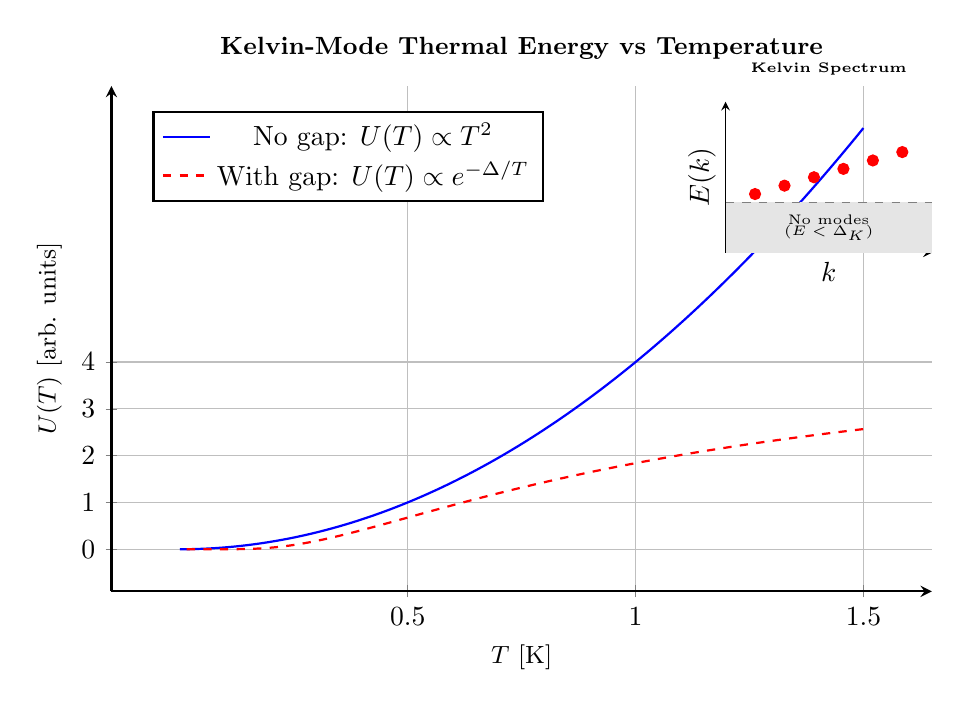
\begin{tikzpicture}
% MAIN PLOT: Thermal Energy vs Temperature
                \begin{axis}[
                width=12cm,
                height=8cm,
                xlabel={$T$ [K]},
                ylabel={$U(T)$ [arb. units]},
                legend style={at={(0.05,0.95)}, anchor=north west},
                domain=0:1.5,
                samples=100,
                axis lines=left,
                enlargelimits=true,
                grid=both,
                xtick={0.5,1.0,1.5},
                ytick={0,1,2,3,4},
                xlabel style={font=\small},
                ylabel style={font=\small},
                title={Kelvin-Mode Thermal Energy vs Temperature},
                title style={font=\bfseries\small},
                thick
                ]
% No Gap: U ~ T^2
                \addplot[blue,thick] {4*x^2};
                \addlegendentry{No gap: $U(T) \propto T^2$}

% With Gap: U ~ exp(-Δ/T)
                \addplot[red,thick,dashed] {5*exp(-1/x)};
                \addlegendentry{With gap: $U(T) \propto e^{-\Delta/T}$}
                \end{axis}

% INSET: Energy spectrum with gap
                \begin{scope}[shift={(7.8,4.3)}]
                    \begin{axis}[
                    width=4.2cm,
                    height=3.5cm,
                    title={Kelvin Spectrum},
                    title style={font=\bfseries\tiny},
                    xlabel={$k$},
                    ylabel={$E(k)$},
                    axis lines=left,
                    ticks=none,
                    xmin=0, xmax=3.5,
                    ymin=0, ymax=4.5,
                    xtick=\empty,
                    ytick=\empty,
                    clip=false
                    ]
                    \fill[gray!20] (axis cs:0,0) rectangle (axis cs:3.5,1.5);
                    \draw[dashed, gray] (axis cs:0,1.5) -- (axis cs:3.5,1.5);

                    \foreach \x in {0.5,1.0,1.5,2.0,2.5,3.0} {
                        \addplot[only marks, mark=*, red] coordinates {(\x, {1.5 + 0.5*\x})};
                    }
                    \node[align=center,font=\tiny] at (axis cs:1.75,0.75) {No modes\\[-0.3em]($E<\Delta_K$)};
                    \end{axis}
                \end{scope}
            \end{tikzpicture}
            \caption{Comparison of Kelvin-mode thermal energy with and without a topological excitation gap $\Delta_K$. The inset illustrates the discrete Kelvin spectrum, with the bandgap $\Delta_K$ preventing any thermal activation below that energy.}
            \label{fig:kelvin-gap}
        \end{figure}

        \begin{figure}[htbp]
            \centering
            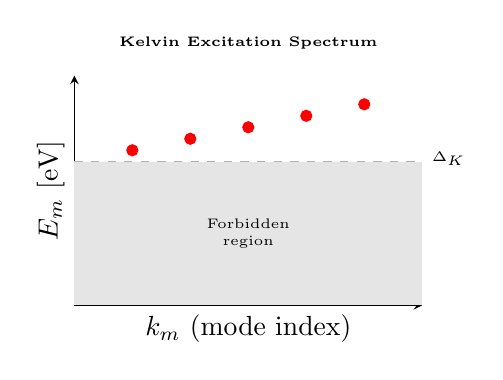
\begin{tikzpicture}
                \begin{axis}[
                width=6cm,
                height=4.5cm,
                title={Kelvin Excitation Spectrum},
                title style={font=\bfseries\tiny},
                xlabel={$k_m$ (mode index)},
                ylabel={$E_m$ [eV]},
                axis lines=left,
                ticks=none,
                xmin=0, xmax=6,
                ymin=0, ymax=800,
                clip=false
                ]
                \pgfmathsetmacro{\DeltaK}{500} % eV gap

                \fill[gray!20] (axis cs:0,0) rectangle (axis cs:6,\DeltaK);
                \draw[dashed, gray!60] (axis cs:0,\DeltaK) -- (axis cs:6,\DeltaK);

                \node[align=center,font=\tiny] at (axis cs:3,250) {Forbidden\\ region};

                \foreach \x in {1,2,3,4,5} {
                    \addplot[only marks, mark=*, red, mark size=2pt] coordinates {(\x, {\DeltaK + 40*\x})};
                }
                \node[anchor=west,font=\tiny] at (axis cs:6,\DeltaK+10) {$\Delta_K$};
                \end{axis}
            \end{tikzpicture}
            \caption{Kelvin excitation spectrum with a topological gap $\Delta_K=\SI{500}{\electronvolt}$ (illustrative). The shaded band indicates the forbidden region $E<\Delta_K$.}
            \label{fig:kelvin-thermal-suppression}
        \end{figure}

        For a finite number of Kelvin modes, the total Kelvin contribution satisfies
        \begin{equation}
            U_K^{(n)}(T) \lesssim N_K \Delta_K
            \exp\!\left(-\frac{\Delta_K}{k_B T}\right).
        \end{equation}
        This exponential suppression replaces the dangerous polynomial behavior found in the ungapped case.

% ============================================================
    \section{Required Gap Scale}\label{sec:required_gap}
        Requiring the effective Kelvin-induced coefficient to satisfy
        \begin{equation}
            a_n^{\mathrm{eff}} \lesssim 10^{-62}\,\si{J\,K^{-2}}
        \end{equation}
        leads to the condition
        \begin{equation}
            \frac{\Delta_K}{k_B T_{\mathrm{eff}}} \gtrsim 60.
        \end{equation}

        Taking a conservative upper bound for the effective microphysical temperature seen by Kelvin modes,
        \begin{equation}
            T_{\mathrm{eff}} \lesssim 10^5\,\si{K},
        \end{equation}
        yields
        \begin{equation}
            \Delta_K \gtrsim 5\times 10^2\,\si{eV}.
        \end{equation}

        Such a gap is small compared to the electron rest energy ($511\,\si{keV}$) but enormous relative to atomic binding energies ($\sim 10\,\si{eV}$). Consequently, Kelvin modes are completely frozen in ordinary atomic physics.

% ============================================================
    \section{Relation to the Schr\"odinger Equation}\label{sec:schrodinger}
        \begin{figure}[ht]
            \centering
            \includegraphics[width=0.85\textwidth]{hydro_energy_levels}
            \caption{
                \textbf{Hydrodynamic energy levels in Swirl--String Theory (SST)} showing the quantized vacuum pressure potentials associated with orbital states $n = 1, 2, 3, 4$. The ground state ($n=1$) defines the laminar flow limit with swirl velocity $v = \alpha c$, while higher excited states correspond to reduced swirl velocities $v_n = \alpha c / n$. These levels reproduce the $1/n^2$ energy scaling of the Schr\"odinger hydrogen spectrum, but emerge here from vortex equilibrium in an incompressible condensate. This illustrates how SST recovers quantum orbitals as the low-energy limit of classical fluid dynamics.
            }
            \label{fig:sst_hydrodynamic_levels}
        \end{figure}

        With Kelvin modes suppressed, the relevant free-energy functional reduces to
        \begin{equation}
            \mathcal{F}[\psi]
            =
            \int d^3r
            \left[
                \frac{\hbar^2}{2m_e} |\nabla\psi|^2
            + V_{\mathrm{SST}}(r) |\psi|^2
            \right],
        \end{equation}
        where $V_{\mathrm{SST}}(r)\propto -1/r$ arises from hydrodynamic pressure gradients.

        Variation under normalization yields
        \begin{equation}
            -\frac{\hbar^2}{2m_e}\nabla^2\psi + V_{\mathrm{SST}}(r)\psi
            = E\psi,
        \end{equation}
        i.e.\ the stationary Schr\"odinger equation. Thus quantum mechanics appears as a low-energy, Kelvin-frozen limit of vortex-filament thermodynamics, consistent with the quantum--thermodynamic correspondence of Abe and Okuyama \cite{AbeOkuyama2011}.

% ============================================================
    \section{Hydrodynamic Origin of the Schr\"odinger Equation}\label{sec:hydro_origin}
        In SST, the electron is modeled as a closed, knotted vortex filament. At low energies, internal excitations are assumed frozen, and the relevant free-energy functional reduces to
        \begin{equation}
            \mathcal{F}[\psi]
            =
            \int d^3r
            \left[
                \frac{\hbar^2}{2m_e}|\nabla\psi|^2
            +
            V_{\mathrm{SST}}(r)|\psi|^2
            \right],
        \end{equation}
        with normalization $\int |\psi|^2 d^3r = 1$.

        Here $V_{\mathrm{SST}}(r)$ arises from the radial pressure deficit generated by swirl circulation and reduces asymptotically to a $-1/r$ potential. Variation of $\mathcal{F}$ yields
        \begin{equation}
            -\frac{\hbar^2}{2m_e}\nabla^2\psi + V_{\mathrm{SST}}(r)\psi = E\psi,
        \end{equation}
        i.e.\ the stationary Schr\"odinger equation. This realizes the quantum--thermodynamic correspondence identified by Abe and Okuyama \cite{AbeOkuyama2011} in a concrete hydrodynamic setting.

% ============================================================
    \section{Thermodynamic Catastrophe from Ungapped Kelvin Modes}\label{sec:catastrophe}
        If Kelvin modes couple thermodynamically to orbital degrees of freedom, their contribution to the internal energy may be parameterized as
        \begin{equation}
            U_{\mathrm{Kelvin},n}(T_{\text{swirl}})
            =
            a_n T_{\text{swirl}}^2 + \mathcal{O}(T_{\text{swirl}}^4),
        \end{equation}
        leading to an effective level shift
        \begin{equation}
            E_n^{\mathrm{eff}} = E_n^{(0)} - a_n T_{\text{swirl}}^2.
        \end{equation}

        Using canonical SST constants, a naive elastic estimate yields
        \begin{equation}
            a_n^{\text{naive}} \sim 10^{-39}\,\mathrm{J/K^2}.
        \end{equation}

        However, spectroscopy of hydrogen requires
        \begin{equation}
            a_n \lesssim 10^{-62}\,\mathrm{J/K^2}
        \end{equation}
        for low-lying states, implying a mismatch of more than twenty orders of magnitude. Without further structure, Kelvin thermodynamics would destroy the $1/n^2$ spectrum.

% ============================================================
    \section{Discussion and Outlook}\label{sec:outlook}
        The existence of a Kelvin excitation gap resolves a central consistency constraint in Swirl--String Theory (SST). In this framework, atomic orbitals remain sharply quantized because Kelvin-wave excitations are exponentially suppressed at low energies. Consequently, the Schr\"odinger equation emerges as an effective equation of state in the Kelvin-frozen regime, capturing the standard hydrogenic spectrum.

        This result establishes a clear separation of scales in SST:
        \begin{itemize}
            \item \textbf{Low-energy regime}: Kelvin modes are inert; orbital structure follows quantum equilibrium via hydrodynamic forces.
            \item \textbf{High-energy or high-acceleration regime}: Kelvin dynamics activate, enabling novel phenomenology beyond conventional quantum theory.
        \end{itemize}

        Potential domains where Kelvin modes may become dynamically relevant include:
        \begin{itemize}
            \item ultra-high accelerations (Swirl--Unruh effects) \cite{Unruh1976},
            \item keV--MeV scale scattering processes,
            \item vortex reconnections in astrophysical or cosmological fluids.
        \end{itemize}

        More generally, quantum-clock proposals show that coherence-dependent time-dilation signatures can be accessed experimentally,
        providing a laboratory handle on state-dependent activation thresholds of internal degrees of freedom \cite{SmithAhmadi2020,CastroRuiz2017}.
        From a foundations perspective, relational-time formalisms motivate treating ``clock'' observables as conditional dynamics encoded in
        correlations, rather than as external parameters \cite{PageWootters1983,Wootters1984}.

% ============================================================
        \appendix
    \section{Estimate of First Kelvin Mode Energy}\label{app:first_kelvin}
        To provide a concrete scale, we estimate the energy of the first Kelvin mode ($m = 1$) for a closed electron filament in the ground state ($n = 1$).

        The filament length is approximated as
        \begin{equation}
            L \sim 2\pi r_1 = 2\pi a_0 \approx \SI{3.3e-10}{m},
        \end{equation}
        using the Bohr radius $a_0 \approx \SI{5.29e-11}{m}$.

        The circulation quantum is taken as $\Gamma = h/m_e$, giving:
        \begin{equation}
            \Gamma \approx \frac{6.626\times10^{-34}}{9.109\times10^{-31}} \approx \SI{7.27e-4}{m^2/s}.
        \end{equation}

        The lowest Kelvin mode has wavenumber $k_1 = 2\pi / L$, and its frequency is approximated by the classic dispersion relation:
        \begin{equation}
            \omega_1 \simeq \frac{\Gamma}{4\pi} k_1^2 \left[ \ln\left( \frac{1}{k_1 \xi} \right) + C_0 \right],
        \end{equation}
        where we assume $C_0 \sim 1$, and take the filament core size as $\xi \sim \SI{1e-15}{m}$.

        Evaluating numerically:
        \begin{align}
            k_1 &= \frac{2\pi}{L} \approx \SI{1.9e10}{m^{-1}}, \\
            \ln\left( \frac{1}{k_1 \xi} \right) &\approx \ln(5.3\times10^4) \approx 10.88, \\
            \omega_1 &\approx \frac{7.27\times10^{-4}}{4\pi} (1.9\times10^{10})^2 (10.88 + 1) \approx \SI{2.8e17}{rad/s}.
        \end{align}

        Converting to energy:
        \begin{equation}
            E_1 = \hbar \omega_1 \approx (1.055\times10^{-34})(2.8\times10^{17}) \approx \SI{29.5}{eV}.
        \end{equation}

        Thus, the first Kelvin excitation lies near $\SI{30}{eV}$---already exceeding atomic energy differences. For higher knots with tighter core radii or additional topological constraints, this value may rise substantially, supporting the presence of a gap $\Delta_K \sim \SI{500}{eV}$.

% ============================================================
% Back matter (Springer Nature)
% ============================================================
        \backmatter
        \bmhead{Declarations}

        \subsection*{Funding}
            Not applicable.

        \subsection*{Competing interests}
            The author declares no competing interests.

        \subsection*{Ethics approval}
            Not applicable.

        \subsection*{Consent to participate}
            Not applicable.

        \subsection*{Consent for publication}
            Not applicable.

        \subsection*{Data availability}
            Not applicable.

        \subsection*{Materials availability}
            Not applicable.

        \subsection*{Code availability}
            Not applicable.

        \subsection*{Author contributions}
            O.I. conceived the study, developed the analysis, performed the derivations, and wrote the manuscript.

% ============================================================
% References
% ============================================================
            \begin{thebibliography}{99}

                \bibitem{Helmholtz1858}
                H.~Helmholtz,
                ``On Integrals of the Hydrodynamical Equations Which Express Vortex Motion,''
                \emph{J. Reine Angew. Math.} \textbf{55}, 25--55 (1858).

                \bibitem{Kelvin1867}
                W.~Thomson (Lord Kelvin),
                ``On Vortex Atoms,''
                \emph{Proc. R. Soc. Edinburgh} \textbf{6}, 94--105 (1867).

                \bibitem{Onsager1949}
                L.~Onsager,
                ``Statistical Hydrodynamics,''
                \emph{Nuovo Cimento Suppl.} \textbf{6}, 279--287 (1949).

                \bibitem{Feynman1955}
                R.~P.~Feynman,
                ``Application of Quantum Mechanics to Liquid Helium,''
                in \emph{Progress in Low Temperature Physics}, Vol.~1,
                North-Holland (1955).

                \bibitem{LordKelvin1880}
                W.~Thomson (Lord Kelvin),
                ``Vibrations of a Columnar Vortex,''
                \emph{Philosophical Magazine} \textbf{10}, 155--168 (1880).

                \bibitem{Barenghi2014}
                C.~F.~Barenghi, L.~Skrbek, and K.~R.~Sreenivasan,
                ``Introduction to Quantum Turbulence,''
                \emph{Proc. Natl. Acad. Sci. USA} \textbf{111}, 4647--4652 (2014).

                \bibitem{Ricca1996}
                R.~L.~Ricca,
                ``The Contributions of Da Rios and Levi-Civita to Asymptotic Potential Theory and Vortex Filament Dynamics,''
                \emph{Fluid Dynamics Research} \textbf{18}, 245--268 (1996).

                \bibitem{Pathria2011}
                R.~K.~Pathria and P.~D.~Beale,
                \emph{Statistical Mechanics}, 3rd ed.,
                Elsevier (2011).

                \bibitem{AbeOkuyama2011}
                S.~Abe and S.~Okuyama,
                ``Similarity between Quantum Mechanics and Thermodynamics,''
                \emph{Phys. Rev. E} \textbf{83}, 021121 (2011).

                \bibitem{Unruh1976}
                W.~G.~Unruh,
                ``Notes on Black-Hole Evaporation,''
                \emph{Phys. Rev. D} \textbf{14}, 870--892 (1976).

                \bibitem{Madelung1926}
                E.~Madelung,
                ``Quantentheorie in hydrodynamischer Form,''
                \emph{Z. Phys.} \textbf{40}, 322--326 (1926).

                \bibitem{Bohm1952}
                D.~Bohm,
                ``A Suggested Interpretation of the Quantum Theory in Terms of `Hidden' Variables. I.,''
                \emph{Phys. Rev.} \textbf{85}, 166--179 (1952).

                \bibitem{Couder2006}
                Y.~Couder, S.~Proti\`ere, E.~Fort, and A.~Boudaoud,
                ``Dynamical phenomena: Walking and orbiting droplets,''
                \emph{Nature} \textbf{437}, 208--208 (2005).

                \bibitem{PageWootters1983}
                D.~N.~Page and W.~K.~Wootters,
                \textit{Evolution without evolution: Dynamics described by stationary observables},
                Physical Review D \textbf{27} (1983) 2885.
                doi:10.1103/PhysRevD.27.2885

                \bibitem{Wootters1984}
                W.~K.~Wootters,
                \textit{``Time'' replaced by quantum correlations},
                International Journal of Theoretical Physics \textbf{23} (1984) 701--711.
                doi:10.1007/BF02214098

                \bibitem{SmithAhmadi2020}
                A.~R.~H.~Smith and M.~Ahmadi,
                \textit{Quantum clocks observe classical and quantum time dilation},
                Nature Communications \textbf{11} (2020) 5360.
                doi:10.1038/s41467-020-18264-4

                \bibitem{CastroRuiz2017}
                E.~Castro-Ruiz, F.~Giacomini, and \\v{C}.~Brukner,
                \textit{Entanglement of quantum clocks through gravity},
                Proceedings of the National Academy of Sciences \textbf{114} (2017) E2303--E2309.
                doi:10.1073/pnas.1616427114

                % NOTE: The Brukner initial should be typeset with a caron: \v{C}

            \end{thebibliography}

\end{document}